%# -*- coding:utf-8 -*-
\subsection[冠状动脉分割II]{改进的基于CURVES的冠状动脉分割}

\begin{frame}
\begin{itemize}
  \item \textbf{心脏区域的VOI提取}:
\end{itemize}
\begin{figure}[t]
\centering
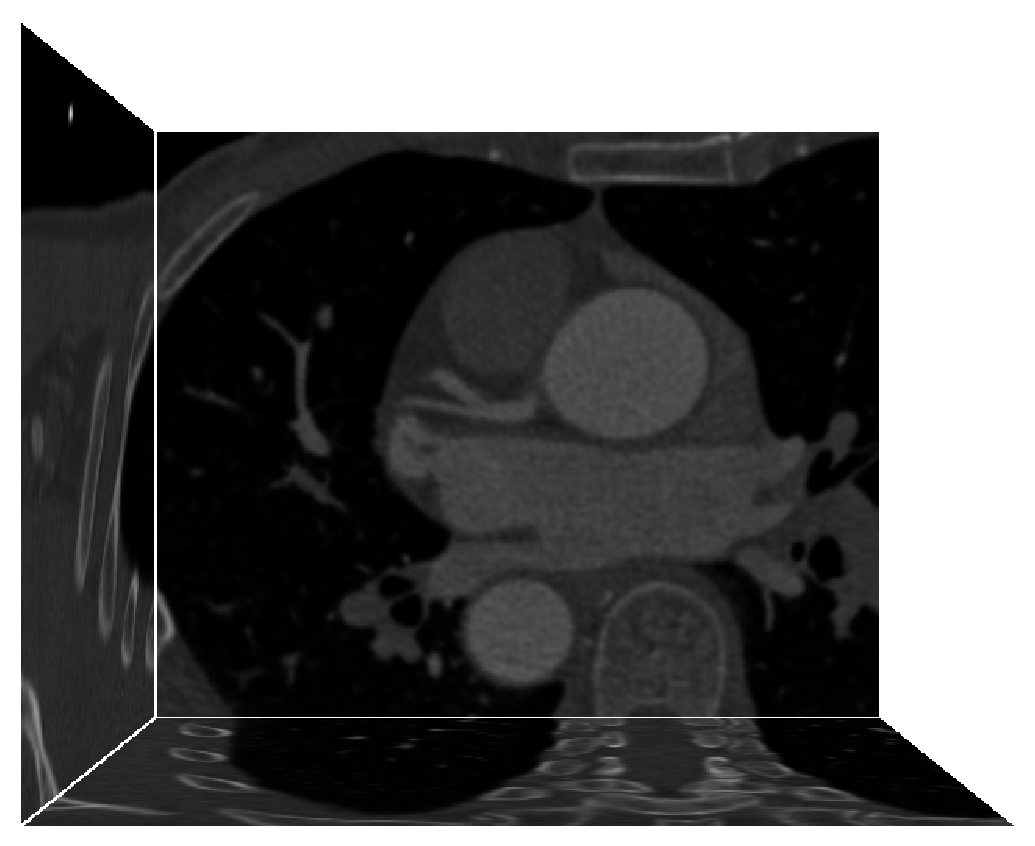
\includegraphics[width=1.5in]{../../Figures/coronary/coronary_enhanced/original}
% \caption[心脏区域的ROI提取]{心脏区域的ROI提取。}
% \label{fig:coronary_ROI}
\end{figure}
\end{frame}

\begin{frame}
\begin{itemize}
  \item \textbf{改进的冠状动脉分割流程}:
\end{itemize}
\begin{figure}[t]
\centering
%# -*- coding:utf-8 -*-
\begin{tikzpicture}[scale=.37]

\draw [black,thick,rounded corners] (-3,0) rectangle (3,2);            % binary threshold
\draw [black,thick,rounded corners] (-3,3) rectangle (3,5);  % CURVES

\draw [black,thick,rounded corners] (-8,7) rectangle (-2,9);   % initial contours

\draw [black,thick,rounded corners] (2,7) rectangle (8,9);     % feature images

\draw [black,thick,rounded corners] (-3,11) rectangle (3,13);  % thresholding
\draw [black,thick,rounded corners] (-3,14) rectangle (3,16);  % curvature anisotropic diffusion
\draw [black,thick,rounded corners] (-3,17) rectangle (3,19);  % raw input

\node [above right] at (-2.25,0.25) {\scriptsize \fs \bf 二值阈值滤波};
\node [above right] at (-2.25,3.25) {\scriptsize \fs \bf 测地活动轮廓};

\node [above right] at (-7.65,7.35) {\scriptsize \fs \bf 初始水平集演进};

\node [above right] at (2.82,7.35) {\scriptsize \fs \bf 特征图像计算};

\node [above right] at (-2.3,11.35) {\scriptsize \fs \bf 二值阈值滤波};
\node [above right] at (-2.9,14.35) {\scriptsize \fs \bf 曲率各向异性扩散};
\node [above right] at (-1.95,17.35) {\scriptsize \fs \bf ROI体数据};

\draw [<-,thick] (0,2) -- (0,3);

\draw [<-,thick] (0,5) -- (0,6);
\draw [thick] (-5,6) -- (5,6);
\draw [thick] (-5,6) -- (-5,7);
\draw [thick] (5,6) -- (5,7);

\draw [<-,thick] (-5,9) -- (-5,10);
\draw [<-,thick] (5,9) -- (5,10);
\draw [thick] (-5,10) -- (5,10);
\draw [thick] (0,10) -- (0,11);

\draw [<-,thick] (0,13) -- (0,14);
\draw [<-,thick] (0,16) -- (0,17);

\end{tikzpicture} 
% 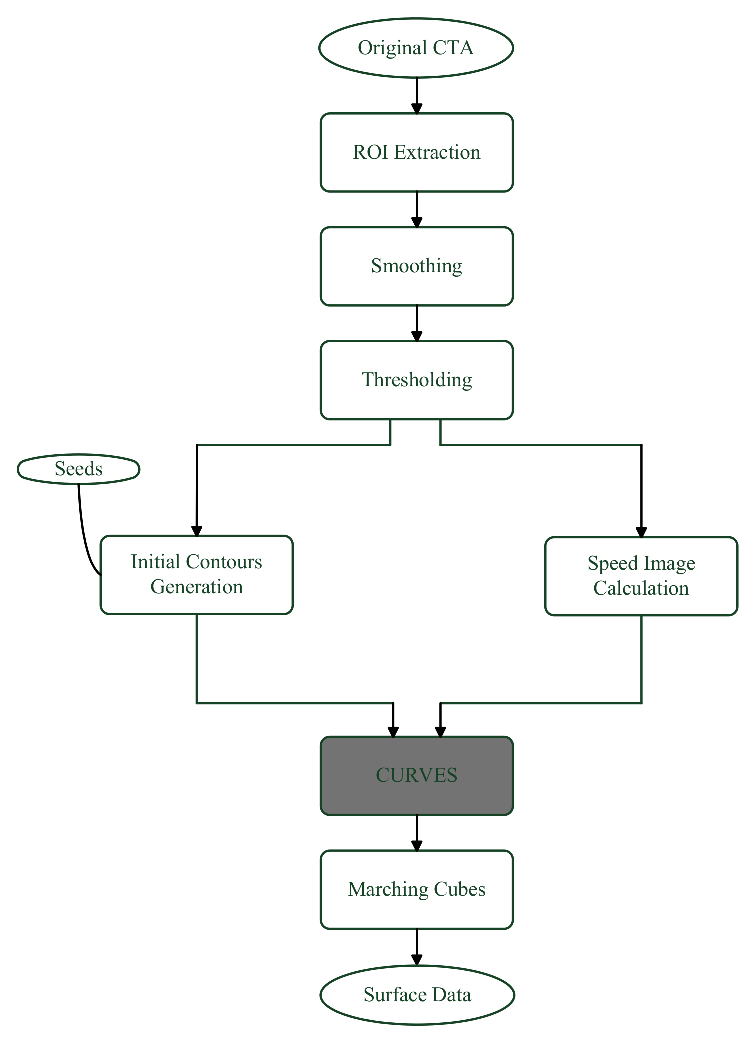
\includegraphics[width=3.2in]{Figures/coronary/DataFlow}
% \caption[心脏区域的ROI提取]{心脏区域的ROI提取。}
% \label{fig:coronary_ROI}
\end{figure}
\end{frame}

\begin{frame}
\begin{itemize}
  \item \textbf{基于vesselness的预处理}:
  \begin{enumerate}
    \item 二值阈值滤波($\text{lower threshold} = 300$, $\text{upper threshold} = 600$)
    \item 管状物体增强($\sigma = 0.9$, $\gamma_{12} = 0.1$, $\gamma_{23} = 2.0$)
  \end{enumerate}
\end{itemize}
\begin{columns}[b,onlytextwidth]
\begin{column}{.5\textwidth}
\begin{figure}[t]
\centering
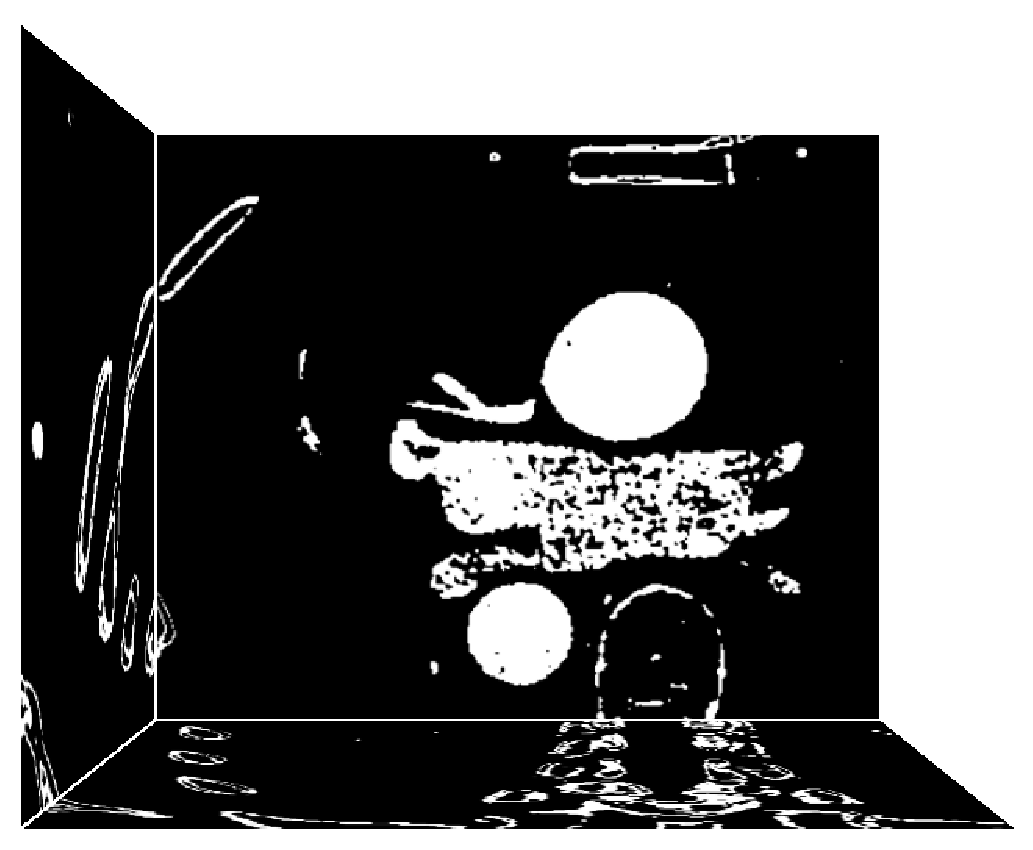
\includegraphics[height=1.5in]{../../Figures/coronary/coronary_enhanced/binary1.eps}
\end{figure}
\end{column}
\begin{column}{.5\textwidth}
\begin{figure}[t]
\centering
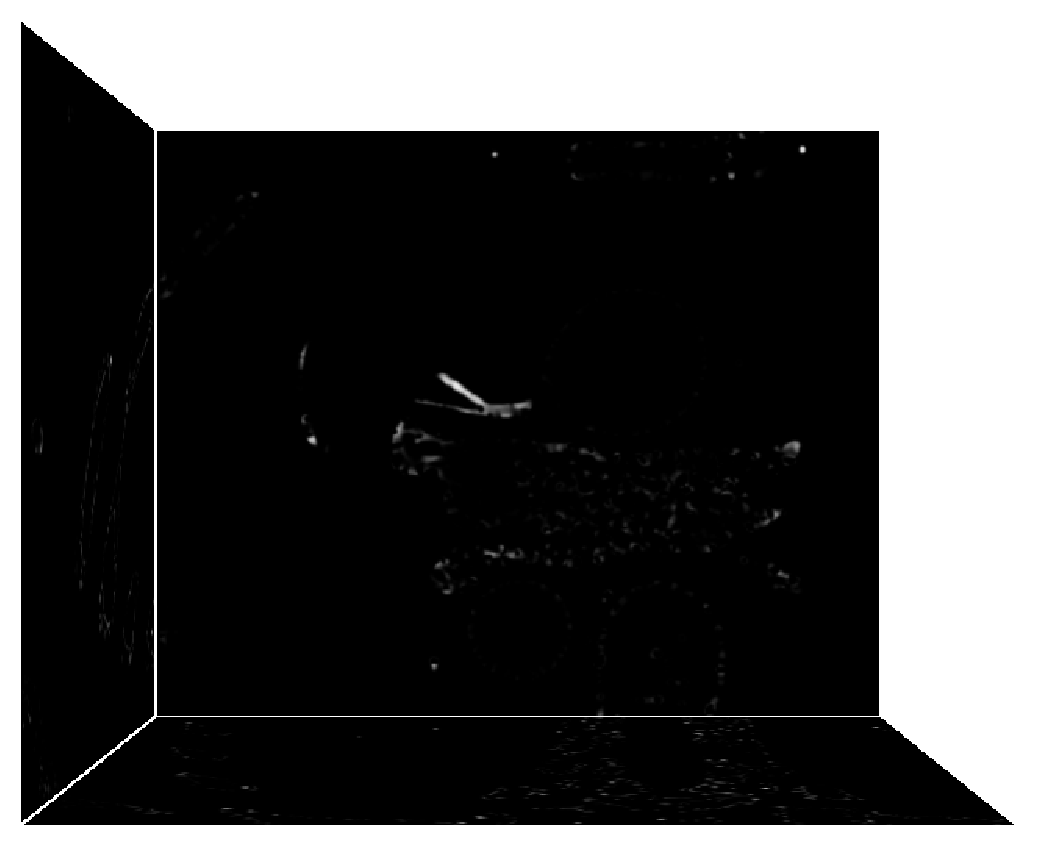
\includegraphics[height=1.5in]{../../Figures/coronary/coronary_enhanced/hessian.eps}
\end{figure}
\end{column}
\end{columns}
\end{frame}

\begin{frame}
\begin{itemize}
  \item \textbf{两种像素亮度处理结果对比}:
  \begin{enumerate}
    \item 非线性亮度映射($m = 80$, $n = 120$)
    \item 二值阈值滤波($\text{TH}_{\text{lower}} = 40$, $\text{TH}_{\text{upper}} = 200$)
  \end{enumerate}
\end{itemize}
\begin{columns}[b,onlytextwidth]
\begin{column}{.5\textwidth}
\begin{figure}[t]
\centering
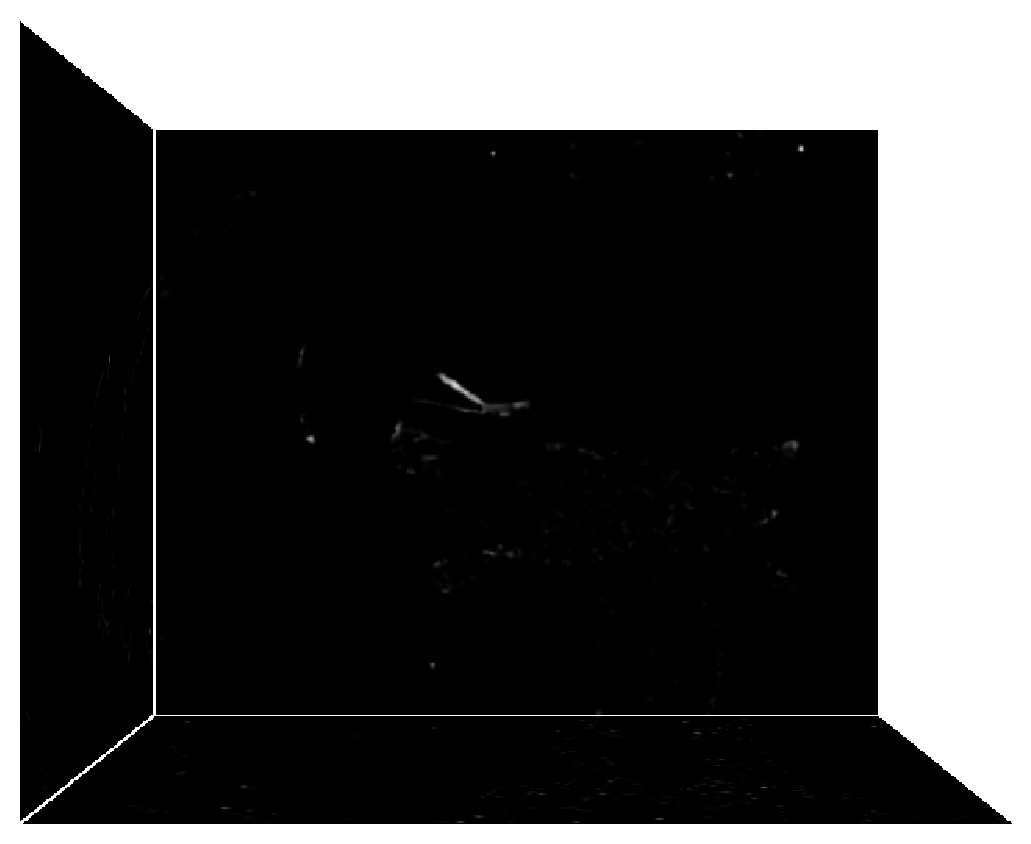
\includegraphics[height=1.5in]{../../Figures/coronary/coronary_enhanced/sigmoid.eps}
\end{figure}
\end{column}
\begin{column}{.5\textwidth}
\begin{figure}[t]
\centering
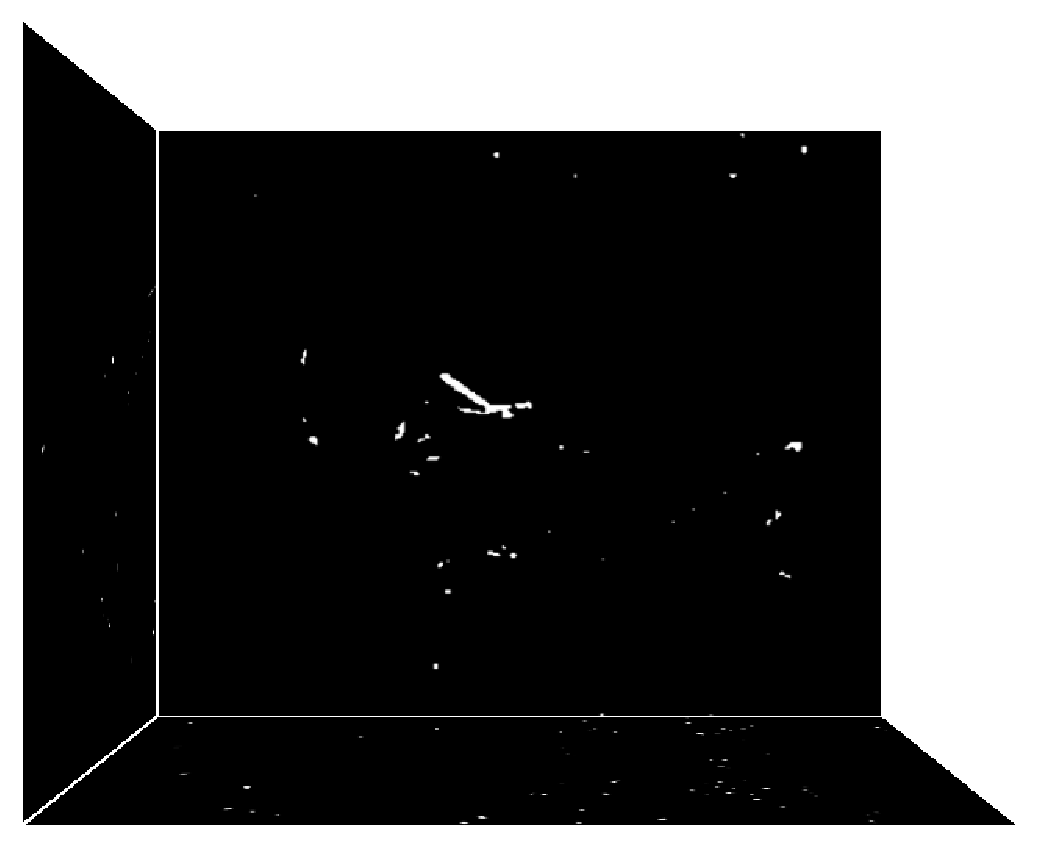
\includegraphics[height=1.5in]{../../Figures/coronary/coronary_enhanced/binary2.eps}
\end{figure}
\end{column}
\end{columns}
\end{frame}

\begin{frame}
\begin{itemize}
  \item \textbf{增强处理后的CURVES演进}:
\end{itemize}
\begin{figure}[t]
\centering

\includegraphics[width=1.5in]{../../Figures/coronary/coronary_enhanced/curves}
% \caption[心脏区域的ROI提取]{心脏区域的ROI提取。}
% \label{fig:coronary_ROI}
\end{figure}
\end{frame}

\begin{frame}
\begin{itemize}
  \item \textbf{冠状动脉模型对比}:
  \begin{enumerate}
    \item 传统CURVES演进
    \item 管状物增强后的CURVES演进
  \end{enumerate}
\end{itemize}
\begin{columns}[b,onlytextwidth]
\begin{column}{.5\textwidth}
\begin{figure}[t]
\centering
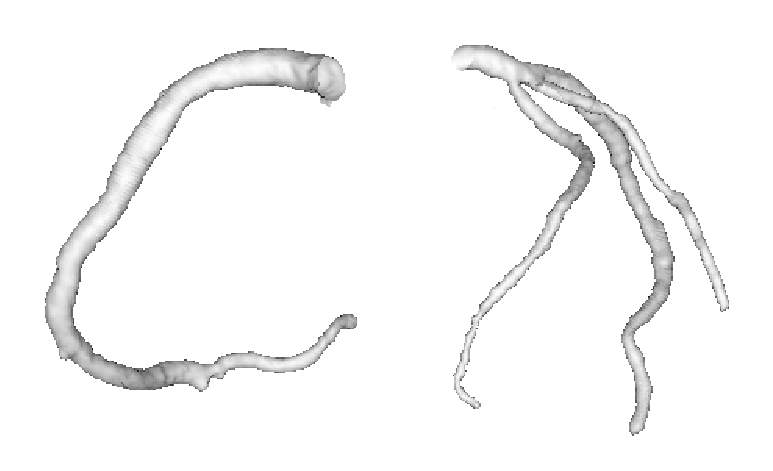
\includegraphics[height=1.5in]{../../Figures/coronary/coronary_enhanced/model_conventional.eps}
\end{figure}
\end{column}
\begin{column}{.5\textwidth}
\begin{figure}[t]
\centering
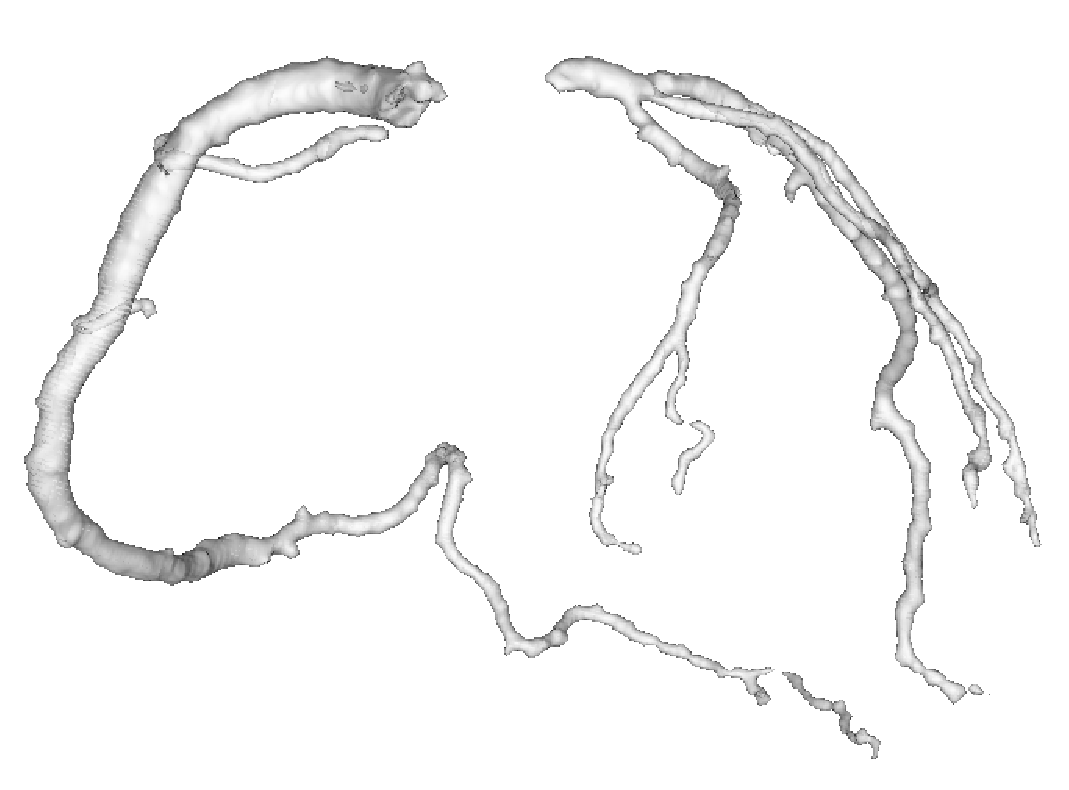
\includegraphics[height=1.5in]{../../Figures/coronary/coronary_enhanced/model_enhanced.eps}
\end{figure}
\end{column}
\end{columns}
\end{frame}

\begin{frame}

\end{frame}

\begin{frame}

\end{frame} 